\documentclass[letterpaper,10pt,titlepage,fleqn]{article}

%example of setting the fleqn parameter to the article class -- the below sets the offset from flush left (fl)
\setlength{\mathindent}{1cm}

\usepackage{graphicx}                                        
\usepackage{amssymb}                                         
\usepackage{amsmath}                                         
\usepackage{amsthm} 
\usepackage{esint}
\usepackage{nopageno}
\usepackage{booktabs}                            
\usepackage{alltt}                                           
\usepackage{float}
\usepackage{color}
\usepackage{fancyhdr}
\usepackage{url}
\usepackage{balance}
\usepackage[TABBOTCAP, tight]{subfigure}
\usepackage{enumitem}
\usepackage{pstricks, pst-node}
%the following sets the geometry of the page
\usepackage{geometry}
\geometry{textheight=9in, textwidth=6.5in}
\pagestyle{fancy}
% random comment
\newcommand{\cred}[1]{{\color{red}#1}}
\newcommand{\cblue}[1]{{\color{blue}#1}}
\usepackage{hyperref}
\usepackage{textcomp}
\usepackage{listings}
\def\name{Best CS325 Group}
%% The following metadata will show up in the PDF properties
\hypersetup{
  colorlinks = true,
  urlcolor = black,
  pdfauthor = {\name},
  pdfkeywords = {cs311 ``operating systems'' files filesystem I/O},
  pdftitle = {Pertinent Information},
  pdfsubject = {Virtual Reality Lab},
  pdfpagemode = UseNone
}

\parindent = 0.0 in
\parskip = 0.2 in
\fboxsep=5mm%padding thickness
\fboxrule=4pt%border thickness

\begin{document}
\lstset{language=Python} 

\title{Programming Assignment \#2 - CS325}

\author{
	Joshua Villwock \and
	Jaron Thatcher \and
	Ryan Phillips
}

\date{February 25, 2014}
\maketitle
%to remove page numbers, set the page style to empty







\section*{Introduction}
\hrule

In this writeup, we will both assess time complexity and prove three algorithms designed to solve the Maximum Subarray problem. 
\par

According to Wikipedia:

\par

`In computer science, the maximum subarray problem is the task of finding the contiguous subarray within a one-dimensional array of numbers (containing at least one positive number) which has the largest sum. For example, for the sequence of values −2, 1, −3, 4, −1, 2, 1, −5, 4; the contiguous subarray with the largest sum is 4, −1, 2, 1, with sum 6.'

\section*{Pseudocode}
\hrule
\begin{centering}

    \textbf{Brute Force:}
    \end{centering}
    \begin{lstlisting}%brute force pseudocode goes here

    def brute_force(x): 
      max_sum = 0
      l = len(x)
      for i in xrange(l):
        new_sum = 0
        for j in range(i,l):
          new_sum += x[j] 
          if new_sum > max_sum: max_sum = new_sum
      return max_sum

    \end{lstlisting}

    \begin{centering}
    \textbf{Divide and Conquer:}
    \end{centering}
    \begin{lstlisting}%divide and conquer pseudocode goes here

    def div_and_conq(x):
      max_sum = 0
      def inner(x,max_sum):    

        if (len(x) <= 1): # base case
          if sum(x) > max_sum:
            max_sum = sum(x)
          return max_sum

        mid = int(len(x)/2) # split into two halves
        l = x[:mid]
        r = x[mid:]

        max_sum = max(max_sum, sum(l)) # is left half max?
        max_sum = max(max_sum, sum(r)) # is right half max?

        # does max consists of suffix+prefix?
        suffix_sum = 0 
        max_suffix_sum = 0
        for i in range(mid-1,-1,-1):
          suffix_sum += x[i]
          max_suffix_sum = max(max_suffix_sum, suffix_sum)
        prefix_sum = 0
        max_prefix_sum = 0
        for i in range(mid,len(x)):
          prefix_sum += x[i]
          max_prefix_sum = max(max_prefix_sum, prefix_sum)
        max_sum = max(max_sum, max_suffix_sum + max_prefix_sum)

        # recursive calls
        ret = inner(l,max_sum) 
        if (ret != None):
          max_sum = max(ret,max_sum)
        ret = inner(r,max_sum)  
        if (ret != None):
          max_sum = max(ret,max_sum)  

        return max_sum # end of inner function

      return inner(x,max_sum)

    \end{lstlisting}

    \begin{centering}
    \textbf{Dynamic Programming:}
    \end{centering}
    \begin{lstlisting}%dynamic programming pseudocode goes here

    def dynamic_prog(x):
      this_sub_arr_sum = 0 
      max_sum = 0
      for i in x:
        if this_sub_arr_sum + i > 0: 
          this_sub_arr_sum = this_sub_arr_sum + i
        else:
          this_sub_arr_sum = 0
        if this_sub_arr_sum > max_sum:
          max_sum = this_sub_arr_sum

      return max_sum

    \end{lstlisting}











\section*{Correctness Proofs}
\hrule

\begin{centering}
\textbf{Divide and Conquer:}
\end{centering}

%divide and conquer proof goes here

TODO

\begin{centering}
\textbf{Dynamic Programming:}
\end{centering}

%dynamic programming proof goes here

TODO

\section*{Asymptotic Analysis of Run Time}
\hrule
\begin{centering}
\textbf{Brute Force:}
\end{centering}

\begin{lstlisting}%brute force asymptotic runtime goes here

TODO

\end{lstlisting}

\begin{centering}
\textbf{Divide and Conquer:}
\end{centering}

\begin{lstlisting}%divide and conquer asymptotic runtime here

TODO

\end{lstlisting}

\begin{centering}
\textbf{Dynamic Programming:}
\end{centering}

\begin{lstlisting}%dynamic programming asymptotic runtime here

\end{lstlisting}

\section*{Empirical Testing of Correctness}
\hrule

Correctness of the three algorithms was verified using the provided file of test cases verify\_2.txt. See the function `test\_correctness' in main.py for details. 

Here is the output from the final text input file (name.txt):

\begin{itemize}
\item OUTPUT HERE (TODO)
\end{itemize}

\newpage

\section*{Empirical Analysis of Run Time}
\hrule
\textbf{Linear Plot:}
\vskip 0.04in
\begin{center}
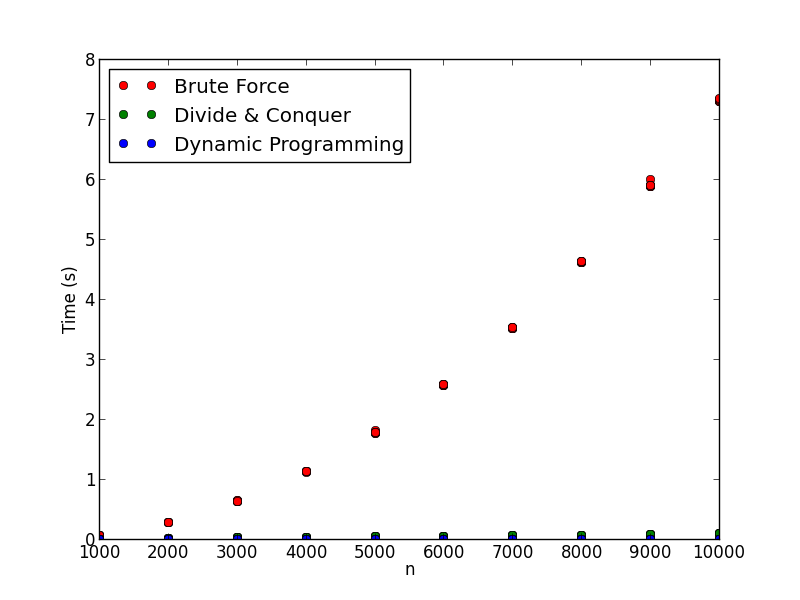
\includegraphics[width=4.5in]{linear.png}
\end{center}
\textbf{Log-log Plot:}
\vskip 0.04in
\begin{center}
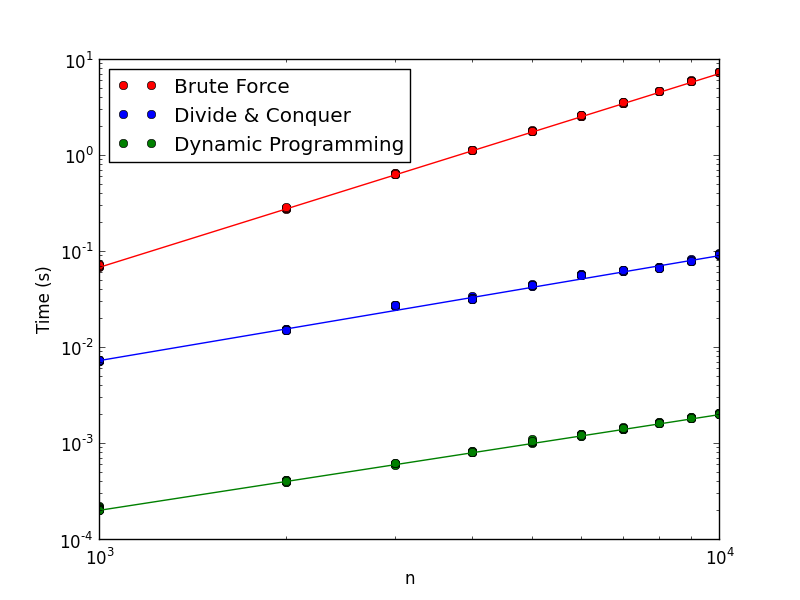
\includegraphics[width=4.5in]{loglog.png}
\end{center}

\newpage

\begin{centering}
\textbf{Slope of lines in log-log plot:}
\end{centering}

The equation for the best fit line on the log-log plot (calculated using numpy.polyfit()) has the following form:

f(n) = e\textsuperscript{y-intercept} * n\textsuperscript{slope}

Brute Force:
\begin{itemize}
\item slope: 2.0177140011
\end{itemize}

Divide \& Conquer:
\begin{itemize}
\item slope: 1.09279503259
\end{itemize}

Dynamic Programming:
\begin{itemize}
\item slope: .996887276493
\end{itemize}

\begin{centering}
\textbf{Performance Comparison}
\end{centering}

Over the range of array sizes under test, Divide and Conquer always performs better than Brute Force, and the Dynamic Programming algorithm always performs better than Divide and Conquer. Sometimes it's necessary to use more temporary memory in order to get performance gains, especially in the case of dynamic programming. But that's not the case here. Some memory usage tests were performed as well, but the results were boring (i.e. no noticeable differences between the algorithms) and don't warrant a graph. 

So in conclusion - for solving the maximum subarray problem, you probably should always use some version of the dynamic programming algorithm presented here.

\end{document}
